\documentclass[10pt,a4paper]{article}
\usepackage[margin=22mm,headheight=14pt]{geometry}
\usepackage[T1]{fontenc}
\usepackage{lmodern,microtype,booktabs,tabularx,graphicx,xcolor,hyperref,fancyhdr,titlesec,tcolorbox,caption}
\definecolor{ink}{HTML}{172B4D}\definecolor{teal}{HTML}{137C8B}\definecolor{coral}{HTML}{E76F51}\definecolor{mist}{HTML}{F1F6F8}
\hypersetup{colorlinks=true,linkcolor=teal,urlcolor=teal}
\setlength{\parindent}{0pt}\setlength{\parskip}{6pt}\setlength{\emergencystretch}{3em}
\pagestyle{fancy}\fancyhf{}\lhead{\textcolor{teal}{IDM-Viz}}\rhead{Phase 3 -- Natural-stream addendum}\cfoot{\thepage}
\titleformat{\section}{\Large\bfseries\color{ink}}{\thesection}{.6em}{}
\captionsetup{font=small,labelfont={bf,color=ink}}
\begin{document}
\begin{titlepage}\color{ink}\vspace*{15mm}
{\large\textcolor{teal}{DATA ANALYSIS AND VISUALIZATION -- PHASE 3}}\\[18mm]
{\Huge\bfseries IDM-Viz}\\[4mm]
{\LARGE NOAA weather-stream transfer addendum}\\[7mm]
{\large A source-verified chronological holdout on Offutt AFB daily records}\\[18mm]
\begin{tcolorbox}[colback=mist,colframe=teal,boxrule=0pt,leftrule=2mm]
\textbf{Evidence boundary}\\
The source is NOAA GSOD, station 72554014949, 1949--1999. The target is same-day rain/drizzle occurrence. This is retrospective classification, not a forward weather forecast.
\end{tcolorbox}
\vfill\textbf{Ahmed Bilal (23I-2581) -- Umar Behram (23I-2604)}\\
FAST-NUCES Islamabad\\[4mm]
Supplementary report -- 17 November 2026\\Editable source: \texttt{REPORT.tex}
\end{titlepage}
\begin{abstract}
This supplement adds a checksum-verified NOAA natural-stream exercise to the controlled IDM-Viz evaluation. A frozen logistic classifier, historical-only scaler/PCA/clusters and isotonic correctness map are fitted on chronological training, calibration and reference segments. The monitoring segment is scored in 21 complete batches of 500 days; 426 remaining rows are disclosed and excluded. Delay-zero labels are replayed only after each batch's scores are persisted. Results are descriptive for one station and one temporal split. They do not identify drift onset, forecast future rainfall, or establish general transfer.
\end{abstract}
\section{Data provenance and admission}
The source is the NOAA/NCEI Global Surface Summary of the Day (GSOD), station \texttt{72554014949}, Bellevue Offutt AFB, Nebraska. The official station-year files cover 1949-01-01 through 1999-12-31. The source manifest records SHA-256 for each of the 51 raw CSV files and for the processed stream. NOAA documents daily summaries and the GSOD fields at \href{https://www.ncei.noaa.gov/metadata/geoportal/rest/metadata/item/gov.noaa.ncdc:C00516/html}{the GSOD metadata page}.

Eight numeric predictors are TEMP, DEWP, SLP, VISIB, WDSP, MXSPD, MAX and MIN. The target is the rain/drizzle bit in FRSHTT. Precipitation and weather-event flags are excluded from predictors. Values are retained in GSOD's reported units. Rows with the documented 999.9 missing code in any selected predictor are dropped. The output has \textbf{18210 days}, from 1949-01-01 through 1999-12-31; positive-label prevalence is 0.316.

The public scikit-multiflow benchmark mirror is retained only as a comparison artifact. Its row count and labels differ from this current timestamped GSOD release, and an exact row-by-row equivalence was not established. It is therefore not used to define timestamps or truth. NOAA's daily summaries include same-day aggregates; consequently this protocol makes no ahead-of-time forecast claim.

\section{Chronological protocol}
The eligible rows are split once, without shuffling: 20\% train (3642), 10\% calibration (1821), 10\% fixed reference (1821) and 60\% monitoring (10926). The 500-row monitor batches span about 500 calendar days each. The final partial cohort of 426 rows is not analyzed. Preprocessing, classifier, PCA, clustering and calibration are frozen after the historical partitions.

At each monitor clock, features are scored and the online CSV is persisted before the evaluator supplies labels to the broker. Delay zero means same batch-clock availability in this replay; it is not a measured operational reporting delay. No delay-5/20 inference is made for NOAA. Released outcomes are kept in evaluator-only files, separate from online scores.

\section{Results}
Table~\ref{tab:estimators} reports equal-weight descriptive summaries over the 21 chronological monitoring batches. Batches are serially dependent; no inferential confidence interval treats them as independent replications.
\begin{table}[ht]
\centering\small\begin{tabular}{lrr}\toprule
Accuracy estimator & Mean batch MAE & Signed bias \\\midrule
Frozen isotonic AC & 0.044 & +0.042 \\
Raw Average Confidence & 0.088 & +0.088 \\
ATC-style threshold & 0.067 & +0.064 \\
Historical constant & 0.044 & +0.036 \\\bottomrule\end{tabular}
\caption{Frozen-model accuracy estimators. Bias is estimate minus observed batch accuracy; negative values indicate underestimation.}\label{tab:estimators}
\end{table}

Mean observed accuracy was 0.751; mean macro-F1 was 0.661 and mean balanced accuracy was 0.654. The calibrated plug-in interval covered 0.429 of batch accuracies, which is weak empirical coverage in this one ordered stream. The historical-constant point estimate slightly outperformed isotonic Average Confidence on mean batch MAE (see Table~\ref{tab:estimators}); calibration is not a universal improvement. The KS/PCA input alarm fired in every monitoring batch, so the result also exposes a high alarm burden under long-run temporal difference from the fixed reference.

\begin{figure}[ht]
\centering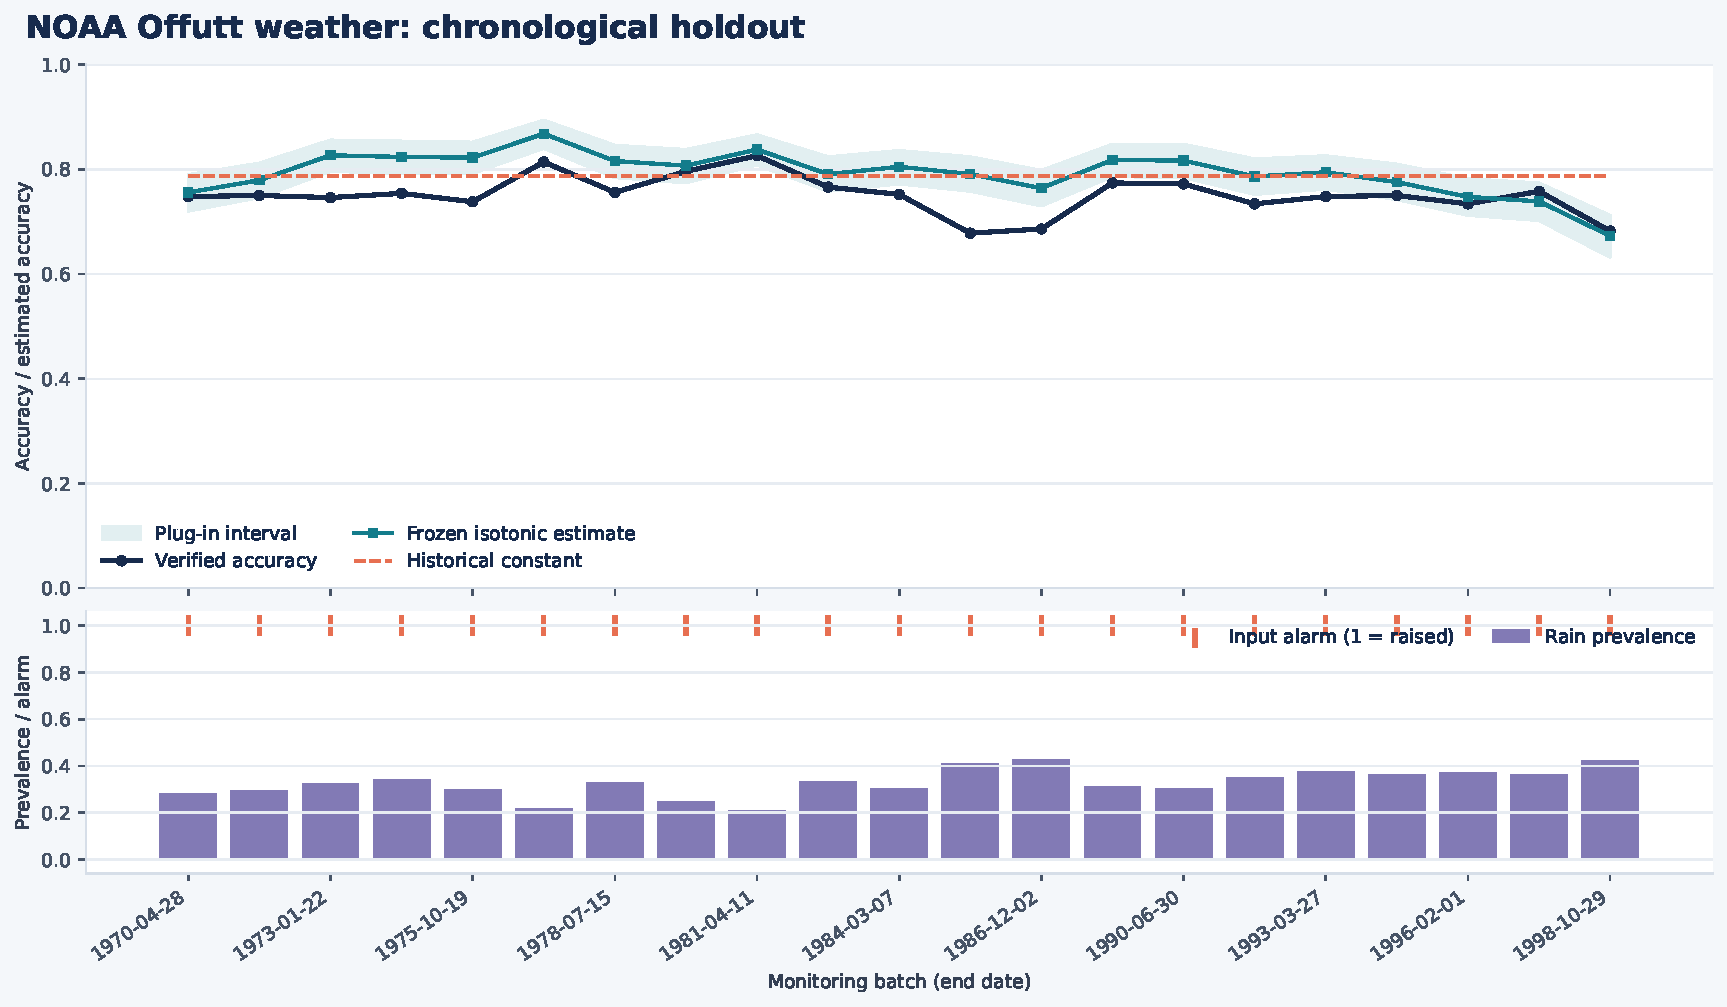
\includegraphics[width=\linewidth]{figures/weather_holdout_timeline.pdf}
\caption{Verified accuracy and frozen estimates by chronological batch. The lower panel shows rain prevalence and input alarms. Dashed/filled elements are descriptive; there is no known change-point truth for this real stream.}
\end{figure}

\section{Interpretation and limits}
This run verifies end-to-end processing on a third natural stream and fixes date/source ambiguity for the weather task. It cannot establish broad domain transfer: all batches come from one station and one chronological split, not independent domains. The 500-day cohorts span long intervals and hide within-batch dynamics. The use of same-day summaries means this is a classification benchmark, not operational early warning. The observed alarm fraction is not false-alarm rate because the natural stream has no known onset labels. Calibration and interval estimates remain conditional on a single historical partition; poor coverage here is an empirical warning, not a population guarantee. No causal, future-risk or analyst-benefit conclusion is supported.

\section{Reproduction}
From the project root with the configured Anaconda environment, run the checked PowerShell reproduction script:
\begin{verbatim}
powershell -ExecutionPolicy Bypass -File scripts/reproduce_noaa_weather.ps1
\end{verbatim}
The script refuses to overwrite its versioned output directories, preprocesses only from the preserved NOAA source files, reruns the frozen chronological evaluation, rebuilds the report and compiles the PDF. Each NOAA source file hash is listed in the manifest. Numerical comparisons should use the saved full-precision CSVs.

\section*{References}
\begin{enumerate}
\item NOAA National Centers for Environmental Information. Global Surface Summary of the Day (GSOD), dataset identifier \texttt{gov.noaa.ncdc:C00516}. \url{https://www.ncei.noaa.gov/metadata/geoportal/rest/metadata/item/gov.noaa.ncdc:C00516/html}.
\item V. Losing, B. Hammer and H. Wersing. \emph{driftDatasets}, Weather description and public benchmark stream. \url{https://github.com/vlosing/driftDatasets}.
\item scikit-multiflow contributors. \emph{streaming-datasets/weather.csv}, legacy benchmark mirror compared in the admission audit. \url{https://github.com/scikit-multiflow/streaming-datasets/blob/master/weather.csv}.
\end{enumerate}
\end{document}
